\section{Animals dataset}

The \textsf{animals} dataset consists of binary values which are the answers to questions such as
"is warm-blooded?", "has lungs?", etc. There are in total 102 such questions, which make up the features, and
33 animal categories, which are the nodes. Figure~\ref{fig:animals} shows the results of estimating the
graph Laplacian of the \textsf{animals} dataset using the \textsf{GGL} algorithm with $\alpha = 0.1$ and
the proposed \textsf{SGL} algorithm with $\beta = 1/2$.

The evaluation of the estimated graphs is done by natural intuition, i.e., we expect that similar animals
such as (\textit{ant}, \textit{cockroach}), (\textit{bee}, \textit{butterfly}), and
(\textit{trout}, \textit{salmon}), would be clustered together, while presently virtually zero connection to
other (group of) animals. Under this sense, it can be seen that the \textsf{SGL} algorithm yields a more intutive
graph than the one learned by \textsf{GGL}.

\begin{figure}[!htb]
    \centering
    \begin{subfigure}[b]{0.475\textwidth}
      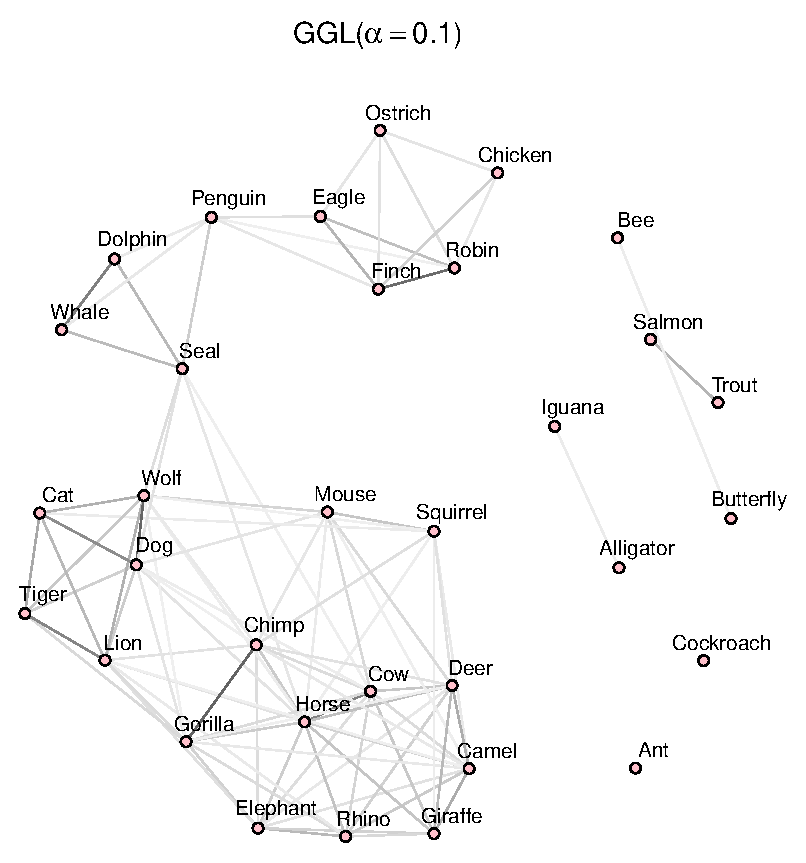
\includegraphics[width=\textwidth]{animals/animals_graph_ggl_alpha01.eps}
      \caption{\textsf{GGL}$(\alpha = 10^{-1})$.}
    \end{subfigure}
    ~
    \begin{subfigure}[b]{0.475\textwidth}
      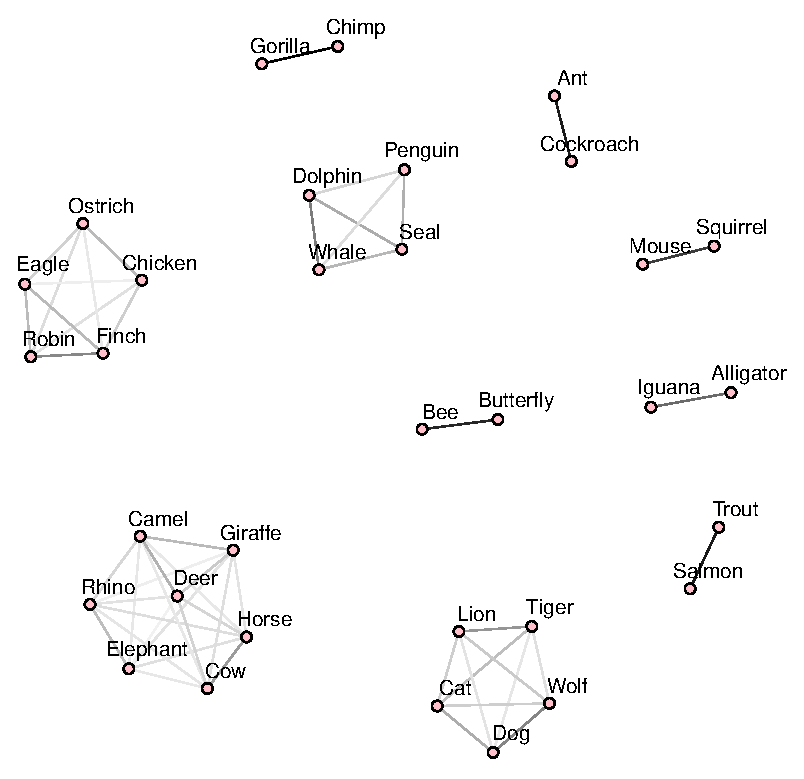
\includegraphics[width=\textwidth]{animals/animals_graph_k10.eps}
      \caption{\textsf{SGL} with $\beta = 1/2$ and $K = 10$.}
    \end{subfigure}
    \caption{Graph structures estimated by (a) \textsf{GGL} and (b) \textsf{SGL} in the \textsf{animals} dataset.}
    \label{fig:animals}
\end{figure}
